%%MaD.tex - Notes taken for Materials and Devices Lecture
%%Author: Andy Goetz
%%Date Modified: 10-7-09
%%License: Ask me before reproducing/modifying, etc.


\documentclass{article}

%Make sure you have the file ShumanNote.scy in the same directory as
%this one. It has contains the style sheet for ECE111, and is needed
%to standardize the layout of LateX documents created for the class.
\usepackage{ShumanNotes} 
\usepackage{tikz}
\usepackage{program}
\usepackage{listings}
\pdfpagewidth 8.5in 
\pdfpageheight 11in

%This package is used to line up pictures 
\usepackage{graphicx}
\usepackage{fancyvrb}
\usepackage{listings}
%allows cursive font
%\usepackage{amsmath}

%allows hyperlinks 
%\usepackage{hyperref}

\newcommand{\HRule}{\rule{\linewidth}{0.5mm}} 

\lhead{T-16 Test Plan}

\begin{document}

%% These commands allow me to use cursive letter for things such as
%% length.  Note that on ubuntu linux, this required installation of
%% the package 'texlive-fonts-extra'. 
%% Taken from
%% http://www.latex-community.org/forum/viewtopic.php?f=5&t=1404&start=0
\newenvironment{frcseries}{\fontfamily{frc}\selectfont}{}
\newcommand{\textfrc}[1]{{\frcseries#1}}
\newcommand{\mathfrc}[1]{\text{\textfrc{#1}}}

\begin{titlepage}
 
\begin{center}
 
 
\textsc{\LARGE Womprat T-16 Audio Synthesizer}\\[1.5cm]
 
\textsc{\Large Portland State University}\\[0.5cm]
 
 
% Title
\HRule \\[0.4cm]
{ \huge \bfseries Test Plan}\\[0.4cm]
 
\HRule \\[1.5cm]
 
% Author and supervisor
\begin{minipage}{0.4\textwidth}
\begin{center} \large
Andy \textsc{Goetz}, Bradon \textsc{Kanyid}, Jackson \textsc{Pugh}, and Kevin \textsc{Riedl}\\
\end{center}
\end{minipage}

 

 
 
\end{center}
\vfill
{ \textit{} }\\[4.0cm]
\begin{center}
% Bottom of the page
{\large \today}

\end{center} 
\end{titlepage}


\section{Overview}

The T-16 Audio Synthesizer is designed to generate an audio output based on multiple channel inputs, as well as tuneable parameters that are controllable from the user interface.  The functionality can be broken down into several independent sub-modules.  These include a microcontroller to synthesize the audio signal, as well as act as a central communications hub for the other sub-modules, a regulated power supply, an EEPROM memory to dynamically store and load pre-defined user settings and miscellaneous data, an LCD to present the user interface, a DAC to convert the synthesizer's digital audio samples into an analog audio output, and an audio amplifier to provide more output power to an internal speaker and offer a master volume control. 

\centerimage{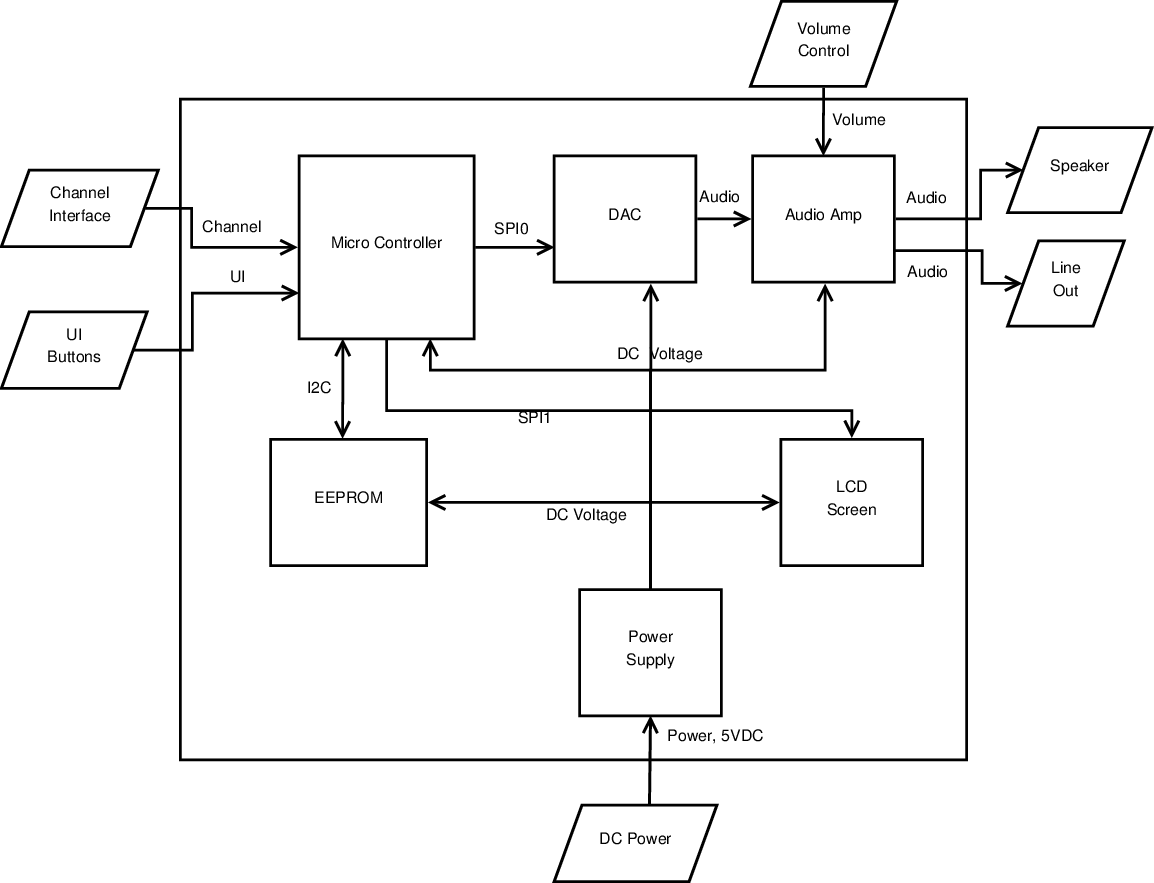
\includegraphics[width=5in]{synth1.png}}{Level 1 Diagram}{fullone}

This document outlines the test approach for the T-16 amplifier. It is
broken down into unit tests, as well as integration and acceptance
tests.

\section{Unit Tests}
\subsection{LCD Tests}
\centerimage{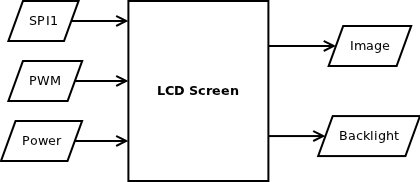
\includegraphics[width=3in]{lcd.png}}{Level 0 Diagram}{LCD}

\begin{tabular}{|p{1in}|p{5in}|}
\hline
\textbf{Module} & LCD \\
\hline
\textbf{Inputs}& SPI: Receives image data from microcontroller.\\
	     & PWM: Backlight brightness control 0-100\% duty cycle.\\
	     & Power: 3.3 VDC Power.\\
\hline
\textbf{Outputs}& Image: Black and white image on 102x64 raster LCD.\\
	      & Backlight: LED light to illuminate the LCD.\\ 
\hline
\textbf{Functionality}& Display the user interface and state of the synthesizer.\\
\hline
\end{tabular}

\subsection{Power Supply Tests}
\centerimage{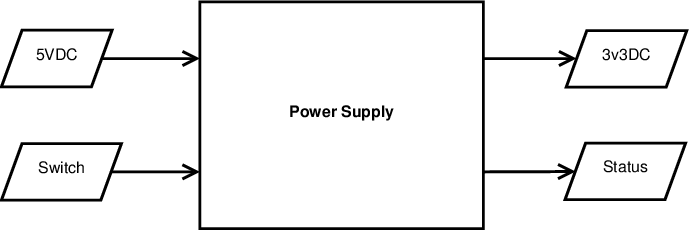
\includegraphics[width=3in]{pwrsply.png}}{Level 0 Diagram}{PSU}

\begin{tabular}{|p{1in}|p{5in}|}
\hline
\textbf{Module} & Power Supply \\
\hline
\textbf{Inputs}& 5VDC: Unregulated power from 5 VDC wall-wart power supply.\\
	     & Switch: On/Off Power Switch.\\
\hline
\textbf{Outputs}& 3v3DC: Regulated 3.3 VDC Power.\\
	      & Status: LED to display if the input power is available.\\ 
\hline
\textbf{Functionality}& The power supply provides regulated 3.3 VDC power to all the subsystems of the audio synthesizer.\\
\hline
\end{tabular}

\subsubsection{Power Supply Overview}
The purpose of the Power Supply is to provide a constant, regulated 3.3 VDC power to the audio synthesizer components.  It includes a 2A protection fuse to limit any high current damage.
\subsubsection{Required Equipment}
\begin{itemize}
\item Audio synth board
\item DC Lab Power Supply
\item Oscilloscope
\end{itemize}
\subsubsection{Fuse Test}
This is a description
\subsubsection{Voltage Ripple Test}
This is a description
\subsubsection{Temperature Test}
This is a description

\subsection{EEPROM Tests}
\centerimage{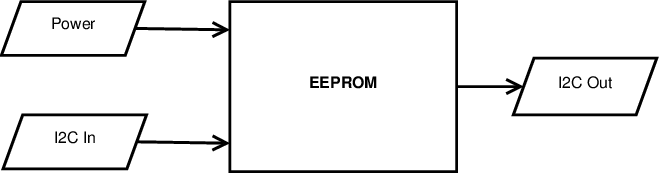
\includegraphics[width=3in]{eeprom.png}}{Level 0 Diagram}{eeprom}

\begin{tabular}{|p{1in}|p{5in}|}
\hline
\textbf{Module} & EEPROM \\
\hline
\textbf{Inputs}& Power: 3.3 VDC Power\\
	     & I2C In: Read data from microcontroller \\
\hline
\textbf{Outputs}& I2C Out: Write data to microcontroller \\ 
\hline
\textbf{Functionality}& Holds user settings for the synthesizer state, as well as the Womprats logo for startup\\
\hline
\end{tabular}
\subsubsection{EEPROM Overview}
The purpose of the EEPROM is to store non-volatile memory so that the Microcontroller can keep settings and store the logo data between power cycles. The Microcontroller talks to the EEPROM via I$^2$C through either burst or byte reads and writes.
\subsubsection{Required Equipment}
\begin{itemize}
\item Audio synth board
\item JTAG programmer for Microcontroller
\end{itemize}
\subsubsection{Write Byte Test}
This is a description
\subsubsection{Write Burst Test}
This is a description
\subsubsection{Read Byte Test}
This is a description
\subsubsection{Read Burst Test}
This is a description

\subsection{Microcontroller Tests}
\centerimage{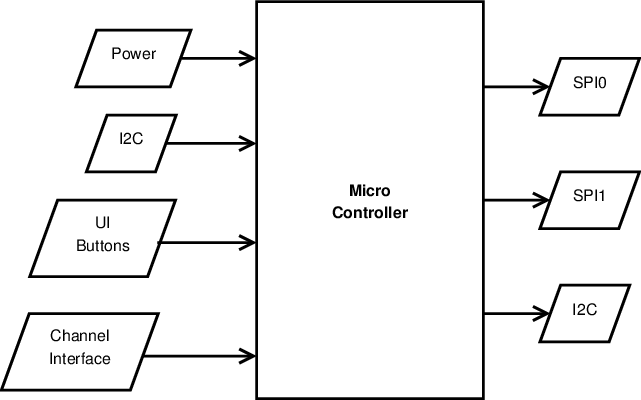
\includegraphics[width=3in]{microcont.png}}{Level 0 Diagram}{micro}

\begin{tabular}{|p{1in}|p{5in}|}
\hline
\textbf{Module} & Microcontroller \\
\hline
\textbf{Inputs}& Power: 3.3 VDC Power\\
	     & I2C: Retrieve data stored in EEPROM\\
	     & UI Buttons: Up/Down/Left/Right/OK/Aux button controls for UI menu interface and entering audio synthesizer settings.\\
	     & Channel Interface: Six analog and digital signal lines that supply parameter control to the audio synthesizer.\\
\hline
\textbf{Outputs}& SPI$_0$: Send digital audio samples to DAC.\\
	      & SPI$_1$: Send image data to LCD.\\
	      & I2C: Store data in EEPROM.\\ 
\hline
\textbf{Functionality}& Implements a software synthesizer that generates an audio signal, shows it's current settings via an LCD screen, is controllable through tunable parameters in the UI and from analog/digital signals on its channel inputs. The tunable parameters are stored in an EEPROM memory that is recalled on startup.\\
\hline
\end{tabular}

\subsection{DAC Tests}
\centerimage{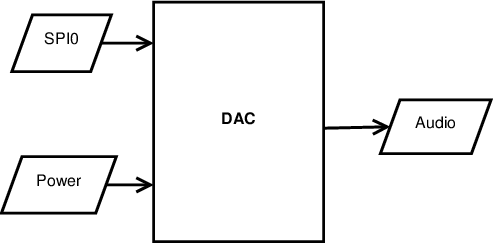
\includegraphics[width=3in]{dac.png}}{Level 0 Diagram}{dac}

\begin{tabular}{|p{1in}|p{5in}|}
\hline
\textbf{Module} & DAC \\
\hline
\textbf{Inputs}& SPI$_0$: Audio samples received from the microcontroller\\
	     & Power: 3.3 VDC power\\
\hline
\textbf{Outputs}& Audio: 0-3.3V audio signal \\ 
\hline
\textbf{Functionality}& The DAC takes the digital audio sample from the microcontroller and converts an analog 0-3.3V audio signal.\\
\hline
\end{tabular}

\subsection{Audio Amplifier Tests}
\centerimage{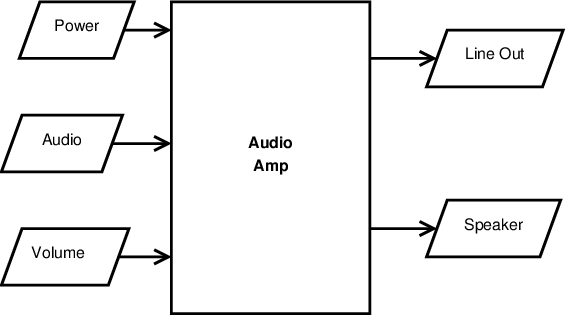
\includegraphics[width=3in]{audioamp.png}}{Level 0 Diagram}{audio}

\begin{tabular}{|p{1in}|p{5in}|}
\hline
\textbf{Module} & Audio Amplifier \\
\hline
\textbf{Inputs} & Power: 3.3 VDC Power\\
	      & Audio: 0-3.3V audio signal from DAC\\
	      & Volume: Controls the audio output volume. Logarithmic control.\\
\hline
\textbf{Outputs}& Line out: Unamplified audio output to external line-out.\\ 
	      & Speaker: Amplified audio output to internal speaker.\\
\hline
\textbf{Functionality}& Provide an amplified audio out that can be heard over the internal speaker or line-out to an external audio device.\\
\hline
\hline
\end{tabular}
\subsubsection{Audio Amplifier Overview}
The purpose of the audio amplifier is to provide an amplified audio signal to the internal speakers or a line-out to an external audio device.  It receives a 0-3.3 VDC signal and has an external volume control to adjust the output volume.  If the line-out is being used, the internal speaker will turn off.
\subsubsection{Required Equipment}
\begin{itemize}
\item Audio synth board
\item DC Lab Power Supply
\item Oscilloscope
\end{itemize}
\subsubsection{Frequency Test}
This is a description
\subsubsection{Headphone Test}
This is a description
\subsubsection{Temperature Test}
This is a description

\section{Integration Tests}


\section{Acceptance Tests}
The primary goal of the T-16 audio amplifier is to demonstrate the
engineering skills of its team members in an interview
situation. Several acceptance tests have been outlined below:

\subsection{Temperature Test}
The completed T-16 Synthesizer must not rise above $10^\circ$ Celsius
while the internal amplifier is in use.
\subsection{Untrained User}
A completely untrained user must be able to make cool sounds with the
T-16 Synthesizer within 5 minutes of picking up the device for the
first time. 

\end{document}
